%
%  Chapter:  1 - Introduction
%  Modified: 2/16/2015
%  Author:   James Till Matta
%
%%%%%%%%%%%%%%%%%%%%%%%%%%%%%%%%%%%%%%%%%%%%%%%%%%%%%%%%%%

\chapter{INTRODUCTION}
\label{chp:intro}
\section{Rotation of Deformed Nuclei}
\label{sec:intro-rot-def-nuc}
Rotation is a universal phenomenon. It exists in the macroscopic world where objects can rotate independently about any set of axes. In the microscopic world of quantum mechanics the situation is more complicated. Rotation about an axis of symmetry is forbidden as the wave function is unchanged. Thus rotation must be about an axes that are not axes of symmetry, limiting it to objects that are deformed, \emph{i.e.} not spherical.

\subsection{Axial Deformation}
\label{ssec:intro-rot-axial-def}
Spherical nuclei are in many ways, exceptional, as Fig. \ref{fig:chp1-quad-def} shows, deformation occurs in many regions of the nuclear chart. In most cases the deformation is slight enough that spherical models can be employed to describe most nuclear properties. However there are regions of the nuclear chart where the deformation grows large enough that it can no longer be ignored. Examples of these regions are the $A\sim{}130$ region and the $A\sim{}170$ region.

\begin{figure}[t!]
\centerline{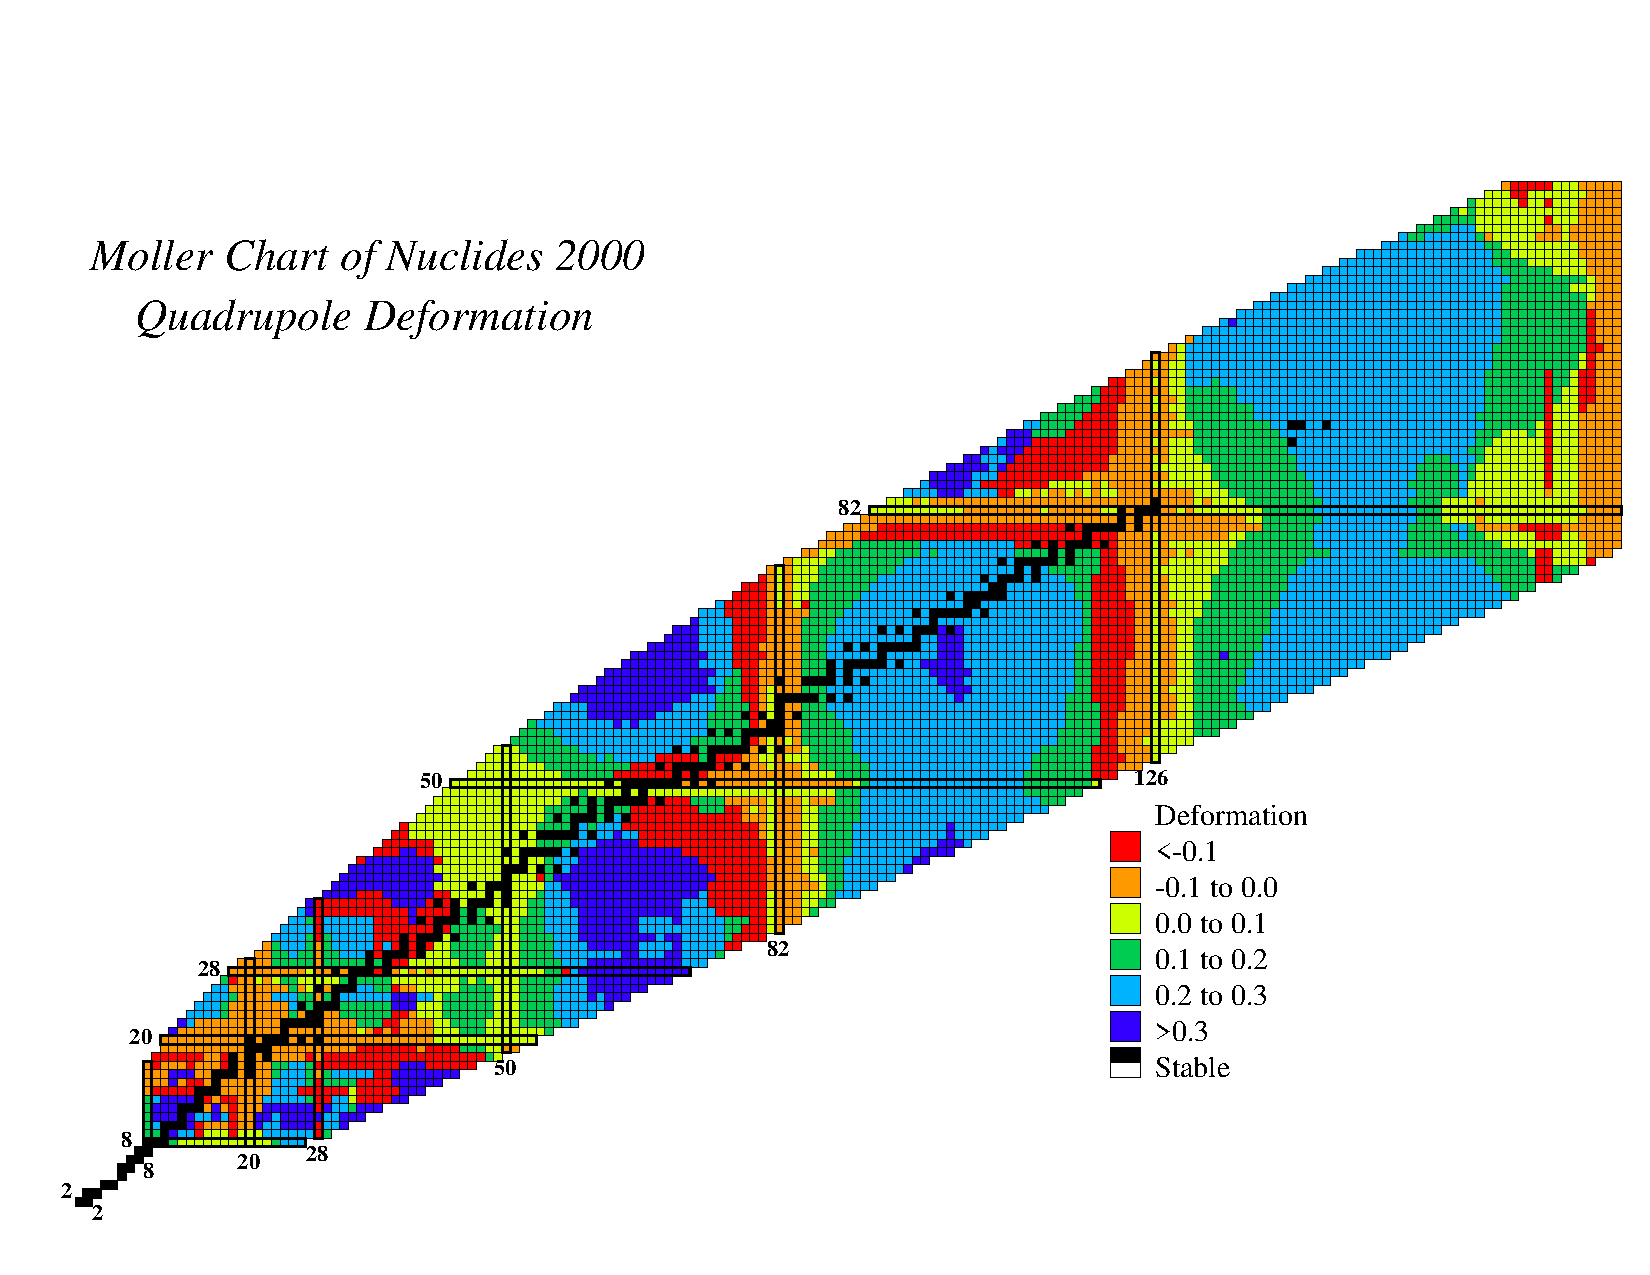
\includegraphics[width=\textwidth,clip=true,trim=0 0 0 75]{./img/c1/chart_thb2.pdf}}
	\caption{Quadrupole deformation parameter $\beta_2$ across the nuclear chart. Plot adapted from \cite{nilssonDiagrams} which used data from \cite{mollerGroundStateDef}.\label{fig:chp1-quad-def}}
\end{figure}

While axial symmetry includes both oblate (pumpkin shaped) and prolate (cigar like) shapes there are quite few oblate nuclei, the majority have prolate deformation. This is usually understood as an effect of single particle structure from the Nilsson model (the Nilsson model is discussed in more detail in Chapter 2). Overall, prolate deformation moves more orbitals to low energy than oblate deformation, therefore in situations where there are several particles a sum over these particles will favor prolate shapes.

\subsection{Triaxiality}
\label{ssec:intro-rot-triax}
Nuclear triaxiality has been a subject of interest for years. While most deformed nuclei are axial in their shape, triaxial shapes have been predicted at low to moderate spin for a few regions of the nuclear chart, \emph{e.g.} Z=60, N=76 and Z=46, N=66  \cite{groundStateTriax}. In searching for triaxiality we are aided by the existence of two unique fingerprints, chirality and wobbling, phenomena that cannot exist unless the nuclear shape is triaxial.

\subsubsection{Chirality}
\label{sssec:intro-rot-chiral}
First predicted in 1997  by S. Frauendorf and J. Meng, chirality occurs when the axis of rotation lies outside the plains spanned by the principal axes of the nucleus \cite{frauendorfChirality,frauendorfTAC,chiralityOfNuclearRotation}. In this configuration the three axes of the nucleus form a screw with respect to the angular momentum vector allowing the construction of two orthogonal configurations with left and right-handed chirality. This manifests itself as pair of nearly degenerate $\Delta{}I=1$ bands with the same parity. Experiment has confirmed the existence of pairs of chiral bands in the $A\sim{}190$, $A\sim{}130$, $A\sim{}100$, and  $A\sim{}80$ regions of the chart of the isotopes, an example from each mass region can be found in Refs. \cite{chiralityIn135Nd,chiralityIn104Rh,chiralityIn80Br,chiralityIn188Ir}

\subsubsection{Wobbling}
\label{sssec:intro-rot-wob}
Of the two fingerprints of nuclear triaxiality, nuclear wobbling was perhaps the longest anticipated. First predicted by A. Bohr and B. Mottelson in Ref. \cite{bohrMottelson2}, wobbling was not observed until the work in 2001 by \O{}deg\aa{}rd \emph{et al.} \cite{wobblingIn163Lu}. Later four more wobbling nuclei were discovered expanding the list to $^{161,163,165,167}$Lu and $^{167}$Ta \cite{wobblingIn163Lu,wobblingIn161Lu,wobblingIn165Lu,wobblingIn167Lu,wobblingIn167Ta}. In the wobbling mode is the quantum mechanical analog of the spinning motion of an asymmetric top. In the high spin limit, where most of the spin is aligned along a principle axis, the wobbling mode is a harmonic vibration describing the precession and nutation of a principal axis of the nucleus about the angular momentum vector.

\subsection{Motivation}
\label{ssec:intro-rot-motivation}
Problematically, while theory predicts an increase for the experimental wobbling energy, given by:
\begin{equation}
\Delta{}E=\hbar\omega_w(I)=E(I,n_w=1)-(E(I-1,n=0)+E(I+1,n_w=0))/2
\end{equation}
to increase with increasing angular momentum, the observed effect is a decrease (see Fig. \ref{fig:chp1-wobbling-freq}). S. Frauendorf and F. D\"{}onau solved this problem with their modified wobbling mode known as ``transverse'' wobbling \cite{frauendorfTransverseWobbling}. Contrary to previous models where the quasiparticle was coupled to the intermediate axis (called ``longitudinal wobbling''), see, for example, Refs. \cite{oldWobblingTheory1,oldWobblingTheory2,oldWobblingTheory3,oldWobblingTheory4}, the quasiparticle is coupled to an axis perpendicular to the intermediate axis. In this model the unpaired quasiparticle couples to the short axis which causes the total angular momentum to wobble about that axis. As angular momentum is added rotation about the medium axis is favored and at some critical angular momentum the motion becomes unstable and the wobbling frequency drops to zero.

The work presented in this dissertation was performed to test the theory of transverse wobbling and show the $A\sim{}130$ region as a viable place to search for the wobbling mode in nuclei.

\begin{figure}[t!]
\centerline{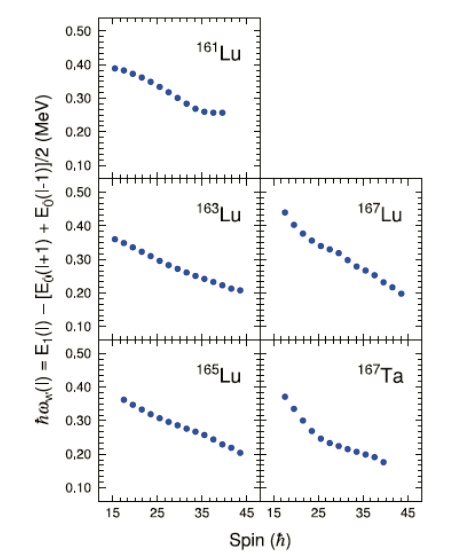
\includegraphics[height=0.3\textheight]{./img/c1/Wobbling_frequencies.png}}
	\caption{Plot of experimental wobbling frequencies for the wobblers in the $A\sim{}170$ mass region.\label{fig:chp1-wobbling-freq}}
\end{figure}
